\documentclass{beamer}
\setbeamertemplate{footline}[frame number]
\usetheme{Ilmenau}
\usecolortheme{dove}
\usepackage{amsmath}
\usepackage{amssymb}
\usepackage{wasysym}
\usepackage{commath}
\usepackage{xcolor}
\definecolor{oxblue}{RGB}{0, 0, 51}
\usepackage{graphicx}
\usepackage{tikz}
\usetikzlibrary{calc}
\usepackage{tkz-euclide}
\usepackage{caption}
\usepackage{subcaption}
\usepackage{float}
\mode<presentation>{}
\usepackage[backend=biber, citestyle=authoryear]{biblatex}
\addbibresource{pres.bib}

\setbeameroption{show notes}

\title{\color{oxblue}{\sc{Stripped Down Cluster Galaxies with Gravitational Lensing}}}
\subtitle{\sc{Part III Presentation}}
\author{\sc{Joe Winterburn}}
\institute{\sc{Institute of Astronomy}}
\date{}



\begin{document}

  \begin{frame}
    \titlepage
  \end{frame}

  \begin{frame}
    \frametitle{\sc Outline}
    \tableofcontents
  \end{frame}

  \section{Background}

  \subsection{Motivations}

  \begin{frame}
    \frametitle{Motivations}
    \begin{itemize}
      \item Lensing directly measures fractional energy density of matter.
      \note{Lensing is a useful probe for $\Omega_m$ in the universe.\\}
      \item Lensing statistics can be used to probe properties of galaxy populations.
      \note{Quantities (convergence, shear, magnification) and statistics (correlation functions, galaxy-galaxy signal) can be computed for galaxy populations.\\}
      \item The effects of tidal stripping in satelite vs central populations can be explored.
      \note{Correlation functions can show differences between these two galaxy populations, and these can be eput into context of the galactic halo model.\\}
      \item Lensing doesn't rely on assumptions about dynamical environment or dark matter distribution.
      \note{Makes it a very useful probe for imaging surveys.\\}
      \item Computing lensing statistics in hydrodynamical simulations and comparing to observation allows constraints to be put on models.
      \note{Some research has been done on this recently, more on that to come.\\}
    \end{itemize}
  \end{frame}

  \begin{frame}
    \begin{itemize}
      \item (\cite{bah2021}) recently explored the claim that cluster subhaloes are more abundant than $\Lambda$CDM predictions.
      \item (\cite{M20}) highlighted this issue and proposed that either there are systematic issues with simulations or incorrect assumptions about dark matter.
      \item (\cite{bah2021}) concludes that there is no tension with $\Lambda$CDM models, but the observed abundances can provide constraints on baryonic physics in simulations.
      \item The take-away is that one needs to be careful about limiting resolution on small scales in cosmological simulations.
    \end{itemize}
  \end{frame}

  \subsection{Horizon AGN}

  \begin{frame}
    \frametitle{\sc Horizon AGN}
    The data made available to me is from the Horizon AGN simulation:
    \begin{itemize}
      \item Cosmological hydrodynamical simulation performed with RAMSES.
      \item $1024^3$ dark matter particles.
      \item Mass resolution of $8\times 10^7 h^{-1} \text{M}_{\astrosun}$.
      \item Lensing quantities (deflection) generated by multiple lens-plane raytracing through the lightcone.
      \note{I believe the raytracing was performed at each simulation time step during the dynamical simulation.\\}
      \item Field of view: 1 deg$^2$ up to $z\approx 7$, 2.25 deg$^2$ up to $z\approx 1$.
      \note{The deep lightcone deflection map is a product of considering 500 transverse lens planes with varying comoving thickness.}
    \end{itemize}
  \end{frame}

  \begin{frame}
    Horizon AGN also provides predictions for flux, based on stars:
    \begin{itemize}
      \item Star properties: mass, age, metallicity $\rightarrow$ spectrum;
      \item These are combined to give a flux prediction. An image of the simulated flux is shown.
    \end{itemize}
    \begin{figure}
      \centering
      \includegraphics[scale=0.3]{figures/hagn/HAGN_img.png}
    \end{figure}
  \end{frame}

  \begin{frame}
    The deflection field is computed from the same gravitational acceleration field used to evolve Eularian quantities in the hydrodynamical simulation. These deflection maps were given to me as the starting point for my work.
    \note{Limitations arise if cells on the boundary of adjacent slabs are updated inbetween the simulation timesteps, but this is rare.\\}
    \begin{itemize}
      \item This is performed recursively for each lens plane.
      \item Goes beyond the Born approximation.
      \note{Born approximation: integrate along straight-line line of sight.}
    \end{itemize}
    \begin{figure}[H]
      \centering
      \includegraphics[width=0.5\textwidth]{figures/hagn/lens-plane-deflection}
    \end{figure}
  \end{frame}

  \subsection{Gravitational Lensing}

  \begin{frame}
    \frametitle{\sc Gravitational Lensing}
    Einstein's General Relativity predicts the gravitational deflection of photons by mass distributions, famously confirmed experimentally by Eddington in 1919.
    \\
    \centering
    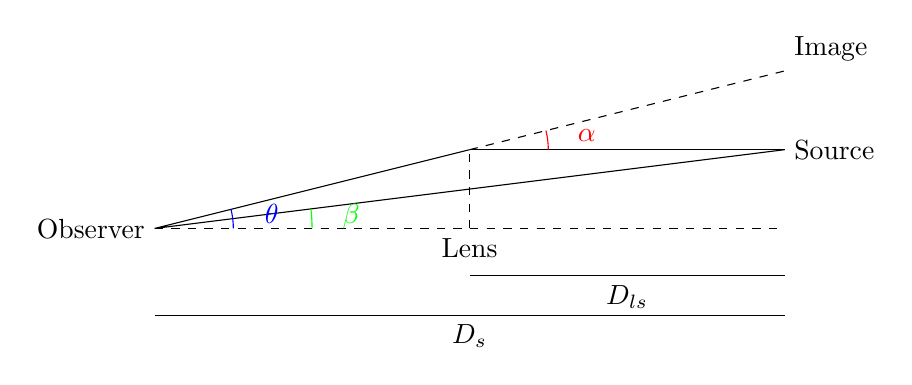
\begin{tikzpicture}
      \coordinate (A) at (-4, 0);
      \coordinate (B) at (0, 0);
      \coordinate (C) at (4, 0);
      \coordinate (D) at (4, 1);
      \coordinate (E) at (4, 2);
      \coordinate (F) at (0,1);

      \draw[thin, black] (F)--(A)--(D);
      \draw[thin, black, dashed] (F)--(E);
      \draw[thin, black] (F)--(D);
      \draw[thin, black, dashed] (B)--(F);
      \draw[thin, black, dashed] (A)--(C);

      \draw (A) node[left] {Observer};
      \draw (B) node[below] {Lens};
      \draw (D) node[right] {Source};
      \draw (E) node[above right] {Image};

      \draw[thin, black] (0, -0.6) -- (4, -0.6) node[midway, below] {$D_{ls}$};

      \draw[thin, black] (-4, -1.1) -- (4, -1.1) node[midway, below] {$D_s$};

      \tkzMarkAngle[blue, opacity=1, size=1](B,A,F);
      \tkzLabelAngle[pos=1.5](B,A,F){$\color{blue}{\theta}$};

      \tkzMarkAngle[red, opacity=1, size=1](D,F,E);
      \tkzLabelAngle[pos=1.5](D,F,E){$\color{red}{\alpha}$};

      \tkzMarkAngle[green, opacity=1, size=2](B,A,D);
      \tkzLabelAngle[pos=2.5](B,A,D){$\color{green}{\beta}$};
    \end{tikzpicture}
  \end{frame}

  \subsection{Weak Lensing}

  \begin{frame}
    The thin lens approximation gives the following relationship between the unobservable true source position $\color{green}{\vec{\beta}}$ and the observed image position $\color{blue}{\vec{\theta}}$:
    \begin{equation} \label{eq:lens}
      \color{green}{\vec{\beta}} \color{black}= \color{blue}{\vec{\theta}} - \color{black}{\frac{D_{\text{ls}}}{D_{\text{s}}}}\color{red}{\vec{\alpha}}\left( \vec{\theta} \right)\color{black}.
    \end{equation}
    \note{This mapping is the basis from which most quantities are derivable. The defelcton angle $\alpha$ is exactly that which is produced by the raytracing. This mapping is also useful for cross referencing lenses to sources in lensing events, as the image positions can be projected into the source plane.}
  \end{frame}

  \begin{frame}
    A Taylor expansion of the lens equation \ref{eq:lens} gives the Jacobian of the $\vec{\theta} \rightarrow \vec{\beta}$ mapping, defining the magnification tensor

    \begin{equation} \label{eq:mu tensor}
      a_{ij}\left( \vec{\theta} \right) = \frac{\partial\vec{\beta}}{\partial\vec{\theta}} = \delta_{ij} - \phi_{,ij} \equiv
      \begin{pmatrix}
        1 - \kappa - \gamma_1 & -\gamma_2 \\
        -\gamma_2 & 1 - \kappa + \gamma_1
      \end{pmatrix}
    \end{equation}

    with $\phi$ the lensing potential, related to the convergence $\kappa$ by $\Delta \phi = \nabla \cdot \vec{\alpha} \equiv 2\kappa$, and $\gamma_{1/2}$ the components of the spin-2 shear.
  \end{frame}

  \begin{frame}
    The lensing observables can be calculated by
    \begin{align} \label{eq:lensing observables}
      \kappa &= \frac{1}{2}\left( \alpha_{1,1} + \alpha_{2,2} \right) \\
      \gamma_1 &= \frac{1}{2}\left( \alpha_{1,1} - \alpha_{2,2} \right) \\
      \gamma_2 &= \alpha_{1,2} = \alpha_{2,1}
    \end{align}
    which can be computed numerically using finite differences.
  \end{frame}

  \begin{frame}
    The convergence is the projected surface mass density in the lens plane expressed in units of the critical density:
    \begin{equation} \label{eq:sigma_kappa}
      \Sigma_{\text{crit}} \kappa\left( \theta \right) = \Sigma\left( \theta \right) = \int\rho\left( \theta, z \right) \dif z.
    \end{equation}

    where the critical density is defined by

    \begin{equation} \label{eq:critical density}
      \Sigma_{\text{crit}} = \frac{c^2}{4\pi G}\frac{D_{s}}{D_{l}D_{ls}}.
    \end{equation}
  \end{frame}

  \begin{frame}
    From (\cite{agn}), the tangential shear, convergence and mean convergence enclosed inside a radius $R$ around a lensing galaxy/halo are related by

    \begin{equation} \label{eq:mean kappa}
      \bar{\kappa}\left( <R \right) = \frac{2}{R^2} \int_0^R \kappa \left( R' \right)R'\dif R' = \kappa \left( R \right) + \gamma \left( R \right).
    \end{equation}

    Using the definition of $\Sigma_{crit}$ in equation \ref{eq:critical density}, the excess density $\Delta\Sigma$ can be defined as

    \begin{equation} \label{eq:delta sigma}
      \Delta\Sigma\left( R \right) = \frac{M\left( <R \right)}{\pi R^2} - \Sigma\left( R \right) = \Sigma_{\text{crit}}\gamma\left( R \right).
    \end{equation}

    So correlation functions can be computed around a selection of lensing galaxies and the statistics can be reated to $\Sigma$ and $\Delta\Sigma$.
  \end{frame}

  \subsection{Strong Lensing}

  \begin{frame}
    In the strong lensing regime, multiple images can be produced from a single source:
    \\
    \centering
    \begin{tikzpicture}
      \coordinate (A) at (-4, 0);
      \coordinate (B) at (0, 0);
      \coordinate (C) at (4, 0);
      \coordinate (D) at (0, 1);
      \coordinate (E) at (0, -1);
      \coordinate (F) at (4, 2);
      \coordinate (G) at (4, -2);

      \filldraw[oxblue] (A) circle (1pt) node[left] {Observer};
      \filldraw[oxblue] (E) circle (1pt) node[below] {Lens};
      \filldraw[oxblue] (C) circle (1pt) node[right] {Source};
      \filldraw[oxblue] (F) circle (1pt) node[right] {Image 1};
      \filldraw[oxblue] (G) circle (1pt) node[right] {Image 2};

      \draw[thin, black, dashed] (A)--(C);
      \draw[thin, black] (A)--(D);
      \draw[thin, black] (A)--(E);
      \draw[thin, black] (D)--(C);
      \draw[thin, black] (E)--(C);
      \draw[thin, black, dotted] (E)--(D);
      \draw[thin, black, dashed] (D)--(F);
      \draw[thin, black, dashed] (E)--(G);
    \end{tikzpicture}
    \\
    \raggedright
    This occurs when light rays pass through a region in which the lensing potential is sufficiently strong.
  \end{frame}

  \begin{frame}
    \begin{itemize}
      \item The mapping $\beta\rightarrow\theta$ is no longer bijective.
      \item Regions in the source plane that correspond to multiple images are caustic regions.
      \item The area of such regions is related to the optical depth for strong lensing $\tau$.
      \item Galaxy catalogs can be projected into the source plane and matched with caustics, allowing cross sections to be related to galactic properties.
    \end{itemize}
  \end{frame}


  \subsection{Limitations}

  \begin{frame}
    \frametitle{\sc Limitations}
    \begin{itemize}
      \item Larger source redshifts mean more potential for noise as the defelction is ofund by integrating along the line of sight, so intermediate matter will feature in the calculation.
      \item Exploring small scales is limited by the resolution of the simulation as mentioned before, and the resolution of the deflection maps.
      \item Isolating galaxies at a range of redshifts means lensing efficiency will vary depending on the distances involved.
    \end{itemize}
  \end{frame}



  \section{Computation and Results}

  \subsection{Weak Lensing: Convergence and Shear}

  \begin{frame}
    \frametitle{\sc Convergence and Shear Maps}
    Convergence and tangential shear maps were computed from the Jacobian of the deflection fields for source redshifts $z_s = 0.39, 1.5, 4.89$ for the narrow 1 deg$^2$ field of view, and $z_s = 0.97$ for the wider 2.25 deg$^2$ field, using finite differences. The resulting maps for the largest redshift in the narrow field, and the wide field are shown:
  \end{frame}

  \begin{frame}
    \begin{figure}[H]
      \centering
      \begin{subfigure}{0.49\textwidth}
        \includegraphics[width=\textwidth]{figures/maps/kappa/kappa_0473.png}
      \end{subfigure}
      \hfill
      \begin{subfigure}{0.49\textwidth}
        \includegraphics[width=\textwidth]{figures/maps/gamma/rebin_gamma_0473.png}
      \end{subfigure}
      \hfill
      \caption{Convergence and tangential shear for $z_s = 4.89$}
      \label{fig:0473 kappa gamma}
    \end{figure}
  \end{frame}

  \begin{frame}
    \begin{figure}[H]
      \centering
      \begin{subfigure}{0.49\textwidth}
        \includegraphics[width=\textwidth]{figures/maps/kappa/kappa_0244.png}
      \end{subfigure}
      \hfill
      \begin{subfigure}{0.49\textwidth}
        \includegraphics[width=\textwidth]{figures/maps/gamma/rebin_gamma_0244.png}
      \end{subfigure}
      \hfill
      \caption{Convergence and tangential shear for $z_s = 0.97$}
      \label{fig:0244 kappa gamma}
    \end{figure}
  \end{frame}

  \begin{frame}
    As the convergence corresponds to the lensing mass distribution, it is instructive to compare the convergence profiles with the simulated light distribution from the simulation:

    \begin{figure}[H]
      \begin{subfigure}{0.49\textwidth}
        \includegraphics[width=\textwidth]{figures/maps/kappa/kappa_0473.png}
      \end{subfigure}
      \hfill
      \begin{subfigure}{0.35\textwidth}
        \includegraphics[width=\textwidth]{figures/hagn/HAGN_img.png}
      \end{subfigure}
      \hfill
    \end{figure}

    A clear correspondence with the convergence map and light distribution can be seen.
  \end{frame}

  \begin{frame}
    Zooming into the main cluster, one can compare the tangential shear to the observed tangential alignment of background sources:

    \begin{figure}[H]
      \begin{subfigure}{0.49\textwidth}
        \includegraphics[width=\textwidth]{figures/maps/gamma/rebin_gamma_0473_zoom.png}
      \end{subfigure}
      \hfill
      \begin{subfigure}{0.35\textwidth}
        \includegraphics[width=\textwidth]{figures/hagn/HAGN-zoom_img.png}
      \end{subfigure}
      \hfill
    \end{figure}
  \end{frame}

  \begin{frame}
    \begin{itemize}
      \item Catalogs of galaxies are provided for the Horizon AGN simulation.
      \item The radial profile of $\kappa$ and $\gamma_t$ were calculated for each galaxy.
      \item Radial bins from $R = 0.02$ Mpc to $R = 5$ Mpc were considered.
      \item Galaxies near the edge of the field of view were excluded as the radial information would be incomplete.
      \item This loss is acceptable as the defelction field is not always well defined near the edge of the field of view due to artefacts arising from the method of calculation within the raytracing step.
    \end{itemize}
  \end{frame}

  \subsection{Radial Profiles}

  \begin{frame}
    Lensing galaxies in small redshift slices are stacked, comparing satellite to central galaxies, and distinguishing stellar mass bins. Some resulting plots are shown below:
  \end{frame}

  \begin{frame}
    \begin{figure}[H]
      \centering
      \includegraphics[width=\textwidth, height=0.8\textheight]{figures/profiles/sigma/0110/0.2-0.3.png}
    \end{figure}
  \end{frame}

  \begin{frame}
    \begin{figure}[H]
      \centering
      \includegraphics[width=\textwidth, height=0.8\textheight]{figures/profiles/delta/0110/0.2-0.3.png}
    \end{figure}
  \end{frame}

  \begin{frame}
    \begin{figure}[H]
      \centering
      \includegraphics[width=\textwidth, height=0.8\textheight]{figures/profiles/sigma/0244/0.2-0.3.png}
    \end{figure}
  \end{frame}

  \begin{frame}
    \begin{figure}[H]
      \centering
      \includegraphics[width=\textwidth, height=\textheight]{figures/profiles/delta/0244/0.2-0.3.png}
    \end{figure}
  \end{frame}

  \begin{frame}
    \begin{figure}[H]
      \centering
      \includegraphics[width=\textwidth, height=0.8\textheight]{figures/profiles/sigma/0308/0.2-0.3.png}
    \end{figure}
  \end{frame}

  \begin{frame}
    \begin{figure}[H]
      \centering
      \includegraphics[width=\textwidth, height=0.8\textheight]{figures/profiles/delta/0308/0.2-0.3.png}
    \end{figure}
  \end{frame}

  \begin{frame}
    \begin{figure}[H]
      \centering
      \includegraphics[width=\textwidth, height=0.8\textheight]{figures/profiles/sigma/0473/0.2-0.3.png}
    \end{figure}
  \end{frame}

  \begin{frame}
    \begin{figure}[H]
      \centering
      \includegraphics[width=\textwidth, height=0.8\textheight]{figures/profiles/delta/0473/0.2-0.3.png}
    \end{figure}
  \end{frame}

  \begin{frame}
    The results are as expected:
    \begin{itemize}
      \item An increase in stellar mass always corresponds to an increase in overall $\Sigma.$
      \item Satellites have a flatter $\Sigma$ and $\Delta\Sigma$ profile at large radii.
      \item The flatter profile and fluctuations in $\Delta\Sigma$ can be put into context of the galactic halo model:
      \begin{itemize}
        \item The $\Delta\Sigma$ profiles peak around the 1-halo term $\left( \Delta\Sigma_{\text{1h}} \right)$ corresponding to the main halo of the host galaxy.
        \item $\Sigma$ profiles are much flatter in the tail as compared to centrals; satellites are expected to reside in the vicinity of a larger halo, so this corresponds to the 2-halo term $\left( \Sigma_{\text{2h}} \right)$.
      \end{itemize}
    \end{itemize}
  \end{frame}

  \subsection{Strong Lensing: Caustics}

  \begin{frame}
    \frametitle{\sc Caustics}
    Caustic maps for the range of source redshifts were computed by exploring the mapping from image to source plane $\theta \rightarrow \beta$. Areas in the source plane onto which multiple image positions are mapped were computed, generating caustic maps of the source plane. An example of such a map is given below:

    \begin{figure}
      \centering
      \includegraphics[width=0.5\textwidth]{figures/caustics/mus_0473.png}
    \end{figure}
  \end{frame}

  \begin{frame}
    Below is a close up of the caustic region corresponding to the largest cluster in the field. Note the astroidal shape, with cusp singularities expected with lensing caustics.

    \begin{figure}
      \centering
      \includegraphics[width=0.5\textwidth]{figures/caustics/closeup_0473.png}
    \end{figure}
  \end{frame}

  \begin{frame}
    \begin{itemize}
      \item Area of caustics $\rightarrow$ optical depth/strong lensing cross section.
      \item Sextractor has been used to build catalogs of individual caustoc regions above a magnification threshold $\left( \mu > 10 \right)$.
      \item Galaxy positions in lens planes are projected into the source plane using the lens equation, and are linked to particular caustic regions.
      \item The most likely caustic region for each lensing galaxy is found using a nearest neighbours algorithm.
    \end{itemize}
  \end{frame}

  \begin{frame}
    \begin{itemize}
      \item The plan is to use this information to relate galactic properties (M$_{*}$, halo environment) to strong lensing cross section. I am yet to carry out this analysis.
      \item An obvious issue that will arise is overcounting of caustic areas due to clustering - this will show up easily in the results and can hopefully be highlighted.
    \end{itemize}
  \end{frame}


\end{document}
